\PassOptionsToPackage{svgnames}{xcolor}
\documentclass[10pt,letterpaper]{article}
\usepackage[top=.25in, bottom=.5in, left=.5in, right=.5in]{geometry}
\usepackage{tcolorbox}
\usepackage{lipsum}
\tcbuselibrary{skins,breakable}
\usetikzlibrary{shadings,shadows}

\usepackage{graphicx} % Allows to include images
\usepackage{booktabs} % Allows the use of \toprule, \midrule and \bottomrule in tables

\usepackage{multicol}
\usepackage{float}

\usepackage[T1]{fontenc}
\usepackage[utf8]{inputenc}

\title{Drills}
\author{}
\date{}

\newenvironment{agendablock}[1]{%
    \tcolorbox[beamer,%
    noparskip,breakable,
    colback=LightGray,colframe=DarkGray,%
    colbacklower=Gray!75!LightGray,%
    title=#1]}%
    {\endtcolorbox}

\newenvironment{evenBlock}[1]{%
    \tcolorbox[beamer,%
    noparskip,breakable,
    colback=LightGreen,colframe=DarkGreen,%
    colbacklower=LimeGreen!75!LightGreen,%
    title=#1]}%
    {\endtcolorbox}

\newenvironment{oddBlock}[1]{%
    \tcolorbox[beamer,%
    noparskip,breakable,
    colback=LightBlue,colframe=DarkBlue,%
    colbacklower=DarkBlue!75!LightBlue,%
    title=#1]}%
    {\endtcolorbox}

\newenvironment{myexampleblock}[1]{%
    \tcolorbox[beamer,%
    noparskip,breakable,
    colback=LightGreen,colframe=DarkGreen,%
    colbacklower=LimeGreen!75!LightGreen,%
    title=#1]}%
    {\endtcolorbox}

\newenvironment{myalertblock}[1]{%
    \tcolorbox[beamer,%
    noparskip,breakable,
    colback=LightCoral,colframe=DarkRed,%
    colbacklower=Tomato!75!LightCoral,%
    title=#1]}%
    {\endtcolorbox}

\newenvironment{myblock}[1]{%
    \tcolorbox[beamer,%
    noparskip,breakable,
    colback=LightBlue,colframe=DarkBlue,%
    colbacklower=DarkBlue!75!LightBlue,%
    title=#1]}%
    {\endtcolorbox}

\usepackage{lmodern}

\begin{document}
\fontfamily{lmss}\selectfont
\maketitle

\section{HOWTO:}
\begin{evenBlock}{HOWTO:  Passing (5 min)}

\begin{minipage}[t]{\linewidth}
    \centering
    Review these elements prior to beginning the passing drills so its fresh in their heads.

    %\begin{minipage}{.3\linewidth} % Left column and width
        %\centering
        %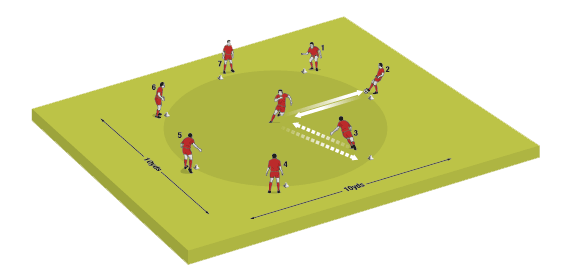
\includegraphics[width=\textwidth]{../img/Trimmed/Clocks1}
    %\end{minipage}
    %\hspace{0.05\linewidth}
    %\begin{minipage}{.6\linewidth} % Left column and width
    
        \textbf{Elements of the Pass:}
    
        \begin{enumerate}
        \setlength{\itemsep}{0pt}
        \setlength{\parskip}{0pt}
        \setlength{\parsep}{0pt}
        \item Ball should start about 1 step in front of the player.
        \item Non-kicking leg should be planted next to the ball with passer's toe pointed at the target.
        \item Ball should be struck in its center,
        \item With the inside portion of the foot.
        \item The kick should follow through.
        \end{enumerate}
        
        \textbf{Elements of the First Touch:}
        \begin{itemize}
        \setlength{\itemsep}{0pt}
        \setlength{\parskip}{0pt}
        \setlength{\parsep}{0pt}
        \item First before the ball is passed be sure you are ready, knees bent and on your toes.
        \item Move your body so the ball is coming directly to you.
        \item Bend your body over the ball as it comes in.
        \item Keep your eye on the ball as it comes into contact with your foot.
        \item Let your foot cushion the ball to slow it down and keep it near your feet.
        \item As your skill develops your first touch can move the ball into the space in which you want (open space or away from the defender).
        \end{itemize}

    %\end{minipage}
\end{minipage}

\end{evenBlock}

\section{Warm Up Drills}

\section{Passing Drills}

\begin{oddBlock}{Lane Passing}

\begin{minipage}[t]{\linewidth}
    \centering
    
    \begin{minipage}{.3\linewidth} % Left column and width
        \centering
        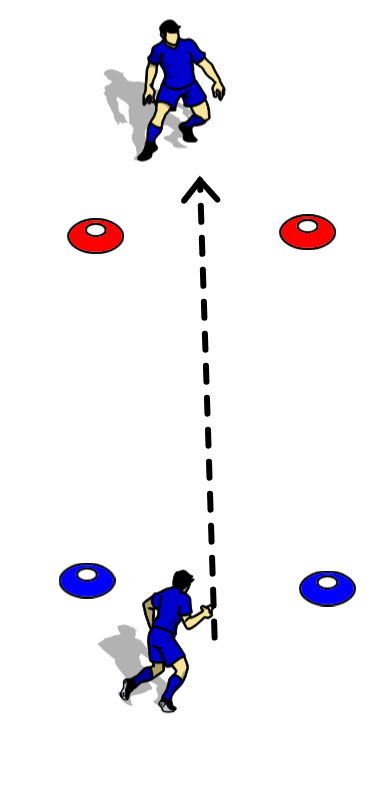
\includegraphics[width=.5\textwidth]{../img/Trimmed/Lane_Pass_BW}
    \end{minipage}
    \hspace{0.05\linewidth}
    \begin{minipage}{.6\linewidth} % Left column and width
        \textbf{Drill Description:}

        \begin{enumerate}
        \setlength{\itemsep}{0pt}
        \setlength{\parskip}{0pt}
        \setlength{\parsep}{0pt}
        \item Two players stand about 5 yards apart.
        \item Players pass the ball to their partner.
        \item The partner tries to two-touch the ball back to their partner.
        \item Alternate passing foot half way through drill.
        \end{enumerate}

        \textbf{Coaching Points:}
        \begin{itemize}
        \setlength{\itemsep}{0pt}
        \setlength{\parskip}{0pt}
        \setlength{\parsep}{0pt}
        \item Focus on passing accurately with pace.
        \begin{itemize}
            \setlength{\itemsep}{0pt}
            \setlength{\parskip}{0pt}
            \setlength{\parsep}{0pt}
            \item Making a single step toward the ball.  This requires the ball to be one step in front of you.
            \item Hitting the center of the ball inside of your foot.
            \item Follow through.
        \end{itemize} 
        \item The goal is to trap the pass using a single touch.
        \item Stay on your toes at all times, this will keep you ready to move.  If you find it hard, focus on bouncing in place.
        \end{itemize}

    \end{minipage}
\end{minipage}

\end{oddBlock}

\begin{oddBlock}{Box Passing (10 min)}

\begin{minipage}[t]{\linewidth}
    \centering
    
    \begin{minipage}{.3\linewidth} % Left column and width
        \centering
        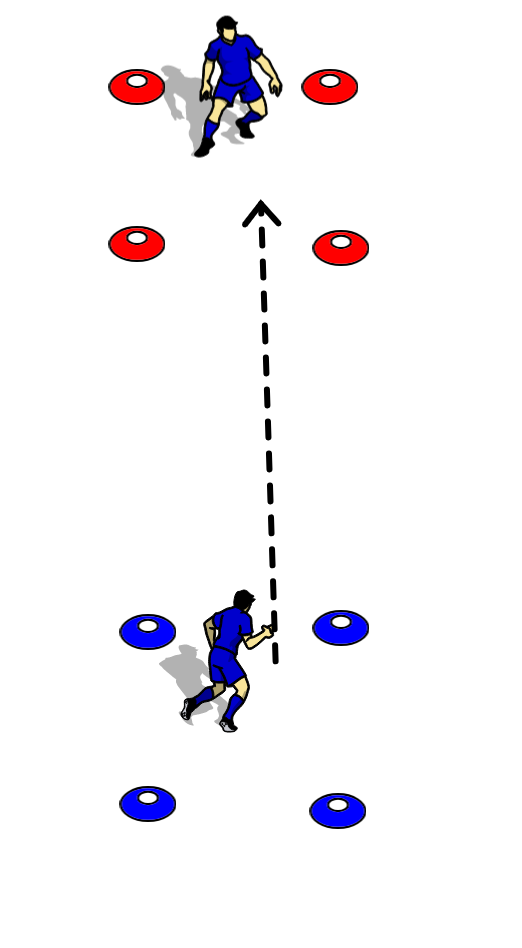
\includegraphics[width=.6\textwidth]{../img/Trimmed/Box_Passing_BW}
    \end{minipage}
    \hspace{0.05\linewidth}
    \begin{minipage}{.6\linewidth} % Left column and width
        \textbf{Drill Description:}

        \begin{enumerate}
        \setlength{\itemsep}{0pt}
        \setlength{\parskip}{0pt}
        \setlength{\parsep}{0pt}
        \item Two players stand in a 2 yard square box.  Boxes should be spaced about 5 yards apart.
        \item Players pass the ball to their partner in the 2 yard box.
        \item The partner tries to trap the ball within the box and pass it back.
        \item Alternate passing \& trapping foot half way through drill.
        \end{enumerate}

        \textbf{Coaching Points:}
        \begin{itemize}
        \setlength{\itemsep}{0pt}
        \setlength{\parskip}{0pt}
        \setlength{\parsep}{0pt}
        \item Focus on passing accurately with pace.
        \begin{itemize}
            \item Making a single step toward the ball.  This requires the ball to be one step in front of you.
            \item Hitting the center of the ball inside of your foot.
            \item Follow through.
        \end{itemize} 
        \item The goal is to trap the pass using a single touch.
        \item Stay on your toes at all times, this will keep you ready to move.  If you find it hard, focus on bouncing in place.
        \end{itemize}

    \end{minipage}
\end{minipage}

\end{oddBlock}

\begin{oddBlock}{Gate Passing (10 min)}

\begin{minipage}[t]{\linewidth}
    \centering
    
    \begin{minipage}{.3\linewidth} % Left column and width
        %\begin{figure}
            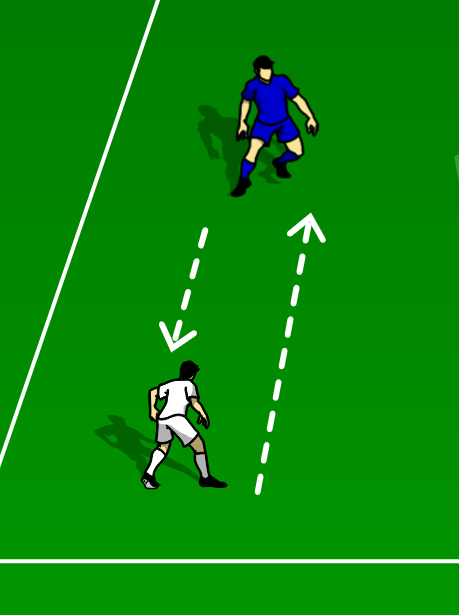
\includegraphics[width=.6\textwidth]{../img/Trimmed/Lane_Passing}
        %    \caption{Drill: 4 Person Passing}
        %\end{figure}
    \end{minipage}
    \hspace{0.05\linewidth}
    \begin{minipage}{.6\linewidth} % Left column and width
        \textbf{Drill Description:}

        \begin{enumerate}
        \setlength{\itemsep}{0pt}
        \setlength{\parskip}{0pt}
        \setlength{\parsep}{0pt}
        \item Two players stand in a 2 yard square box.  Boxes should be spaced about 5 yards apart.
        \item Players pass the ball to their partner in the 2 yard box.
        \item The partner tries to trap the ball within the box and pass it back.
        \end{enumerate}

        \textbf{Coaching Points:}
        \begin{itemize}
        \setlength{\itemsep}{0pt}
        \setlength{\parskip}{0pt}
        \setlength{\parsep}{0pt}
        \item Focus on passing accurately with pace.
        \item The goal is to trap the pass using a single touch.
        \end{itemize}

    \end{minipage}
\end{minipage}

\end{oddBlock}

\begin{evenBlock}{Four Corner Passing}

\begin{minipage}[t]{\linewidth}
    \centering
    
    \begin{minipage}{.3\linewidth} % Left column and width
        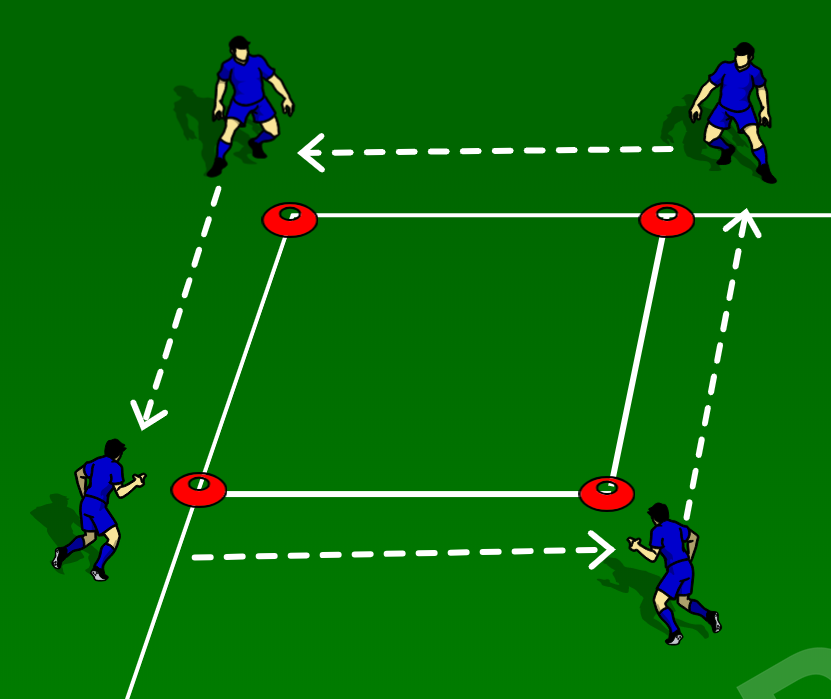
\includegraphics[width=.8\textwidth]{../img/Trimmed/Triangle_Passing_4P_mini}
    \end{minipage}
    \hspace{0.05\linewidth}
    \begin{minipage}{.6\linewidth} % Left column and width
        \textbf{Drill Description:}
        This drill focuses only on passing accurately and using the correct foot for the first touch.  This is like a 3 man passing drill around a box, but with an extra man so there is no movement element which should allow them to focus on the proper technique.
        \begin{enumerate}
            \setlength{\itemsep}{0pt}
            \setlength{\parskip}{0pt}
            \setlength{\parsep}{0pt}
            \item All players stand `open' to they can see all 3 of the players.
            \item The ball should be passed on one direction to start (to the left is more natural for a right footed player).
            \item The player receiving the ball should move his body so he receives the ball on his left foot then passes it to the next player using his right.
            \item After 5 rounds around the box, switch directions.  Pass to the right using the left foot, trap with the right.
        \end{enumerate}
    \end{minipage}

        \raggedright
        \textbf{Coaching Points:}
        \begin{itemize}
            \setlength{\itemsep}{0pt}
            \setlength{\parskip}{0pt}
            \setlength{\parsep}{0pt}
            \item Explain the first touch with the correct foot is the most important part.
            \item The touch should place the ball one step away from the player so they can step into and make a strong pass.
            \item The goal is to use two touches, not 1 and not 3.
            \item Once the passing and trapping with the correct foot becomes more natural, allow then to change directions at will, but any two adjacent players can't pass the ball back and forth more than 3 times.
        \end{itemize}

    
\end{minipage}

\end{evenBlock}

\begin{evenBlock}{Triangle Passing}
\textbf{Drill Description:}
        This drill is like the `4 Corner Passing Drill' but incorporates player movement to insure the player with the ball always has two options to pass too.
        If the groups are uneven, a `defender' can be added to the box.  If the pass goes through the box the passer switches location with the defender.  If trap is on the wrong foot the trapper switches with the defender.  Defenders count 5 successful passes and they switch with a player.
\begin{minipage}[t]{\linewidth}
    \begin{minipage}{.3\linewidth} % Left column and width
        \centering
        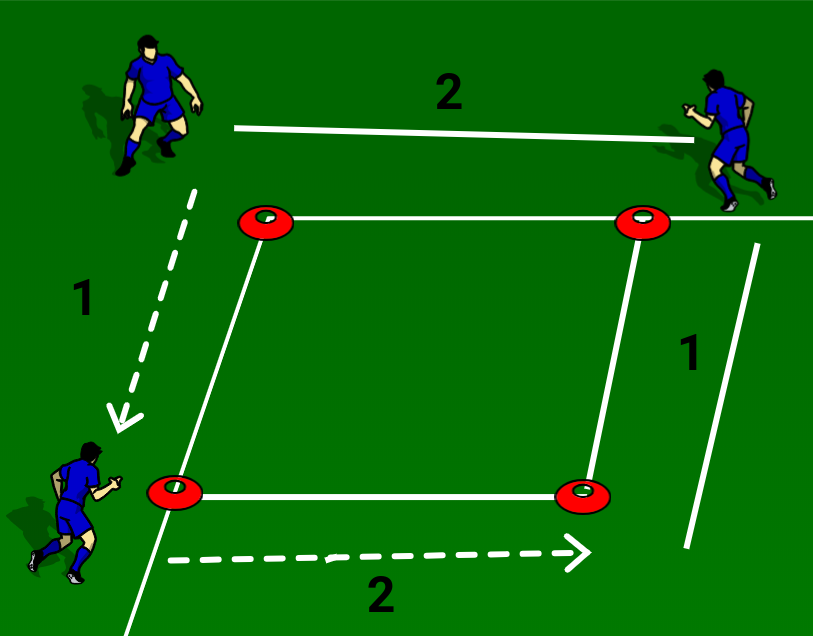
\includegraphics[width=\textwidth]{../img/Trimmed/Triangle_Passing_3P_mini}
    \end{minipage}
    \hspace{0.05\linewidth}
    \begin{minipage}{.6\linewidth} % Left column and width
        \begin{enumerate}
            \setlength{\itemsep}{0pt}
            \setlength{\parskip}{0pt}
            \setlength{\parsep}{0pt}
            \item All players stand `open' so they can see the other two players.
            \item The ball should be passed on one direction to start (to the left is more natural for a right footed player).
            \item The player receiving the ball should move his body so he receives the ball on his left foot then passes it to the next player using his right.  However the pass should wait until the 3 player is in position.
            \item  Player 3 (P3) was at a corner nearest the ball, however once the ball was passed, P3 needs to move to the other corner so they are again at a corner adjacent to the player with the ball.
            \item After 5 rounds around the box, switch directions.  Pass to the right using the left foot, trap with the right.
            \item After 5 additional rounds allow the player to switch directions at will, but any two adjacent players can't pass the ball back and forth more than 3 times.
        \end{enumerate}
    \end{minipage}
\end{minipage}
\raggedright
    \textbf{Coaching Points:}
    \begin{itemize}
        \setlength{\itemsep}{0pt}
        \setlength{\parskip}{0pt}
        \setlength{\parsep}{0pt}
        \item Explain the first touch with the correct foot is the most important part.
        \item The touch should place the ball one step away from the player so they can step into and make a strong pass.
        \item The goal is to use two touches, not 1 and not 3.
    \end{itemize}

\end{evenBlock}

\begin{evenBlock}{Figure 8 Passing (10 min)}

\begin{minipage}[t]{\linewidth}
    \centering
    
    \begin{minipage}{.3\linewidth} % Left column and width
        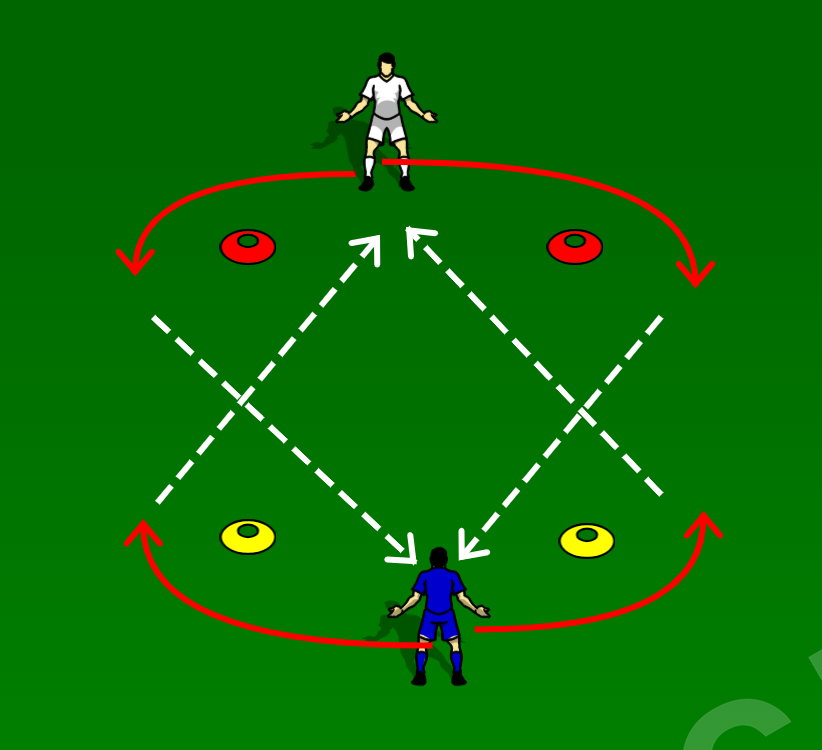
\includegraphics[width=\textwidth]{../img/Trimmed/Figure-8}
    \end{minipage}
    \hspace{0.05\linewidth}
    \begin{minipage}{.6\linewidth} % Left column and width
        \textbf{Drill Description:}
        This drill incorporates a lot of movement and passing.  Its designed to make the player trap and touch a ball around a defender for a clear pass.
        \begin{enumerate}
            \setlength{\itemsep}{0pt}
            \setlength{\parskip}{0pt}
            \setlength{\parsep}{0pt}
            \item Player 1 starts with the ball between two cones.  P2 starts between two cones the same width apart as P1 and 5 yards away.
            \item P1 dribbles around the cone on the right and passes to P2.
            \item P2 should trap the ball with the right foot and dribble around the right cone and pass to P1, who needs to race back between the two cones.
            \item This time P1 traps with the left foot and dribbles around the left cone and passes to P2.  P2 needs to race back between the two cones.
            \item P2 traps with the left and dribbles around the left cone to pass back to P1.
            \item At this point the drill repeats to the right side.
            \item After 10 passes stop and the P2 becomes the starting player.
        \end{enumerate}
    \end{minipage}
\end{minipage}

\textbf{Coaching Points:}
\begin{itemize}
    \setlength{\itemsep}{0pt}
    \setlength{\parskip}{0pt}
    \setlength{\parsep}{0pt}
    \item The cones are the defender, the goal is practice making that first touch and follow on touches into the open space then pass.
    \item Explain the first touch with the correct foot is important in guiding the ball into the open space.
    \item The goal would be able to use only 2 touches before making that third touch (the pass). 
    \item However I would rather see 3, 4 or 5 tight controlled touches than only 2 sloppy touches.

\end{itemize}


\end{evenBlock}

\begin{evenBlock}{Clocks (10 min)}

\begin{minipage}[t]{\linewidth}
    \centering
    
    \begin{minipage}{.3\linewidth} % Left column and width
        \centering
        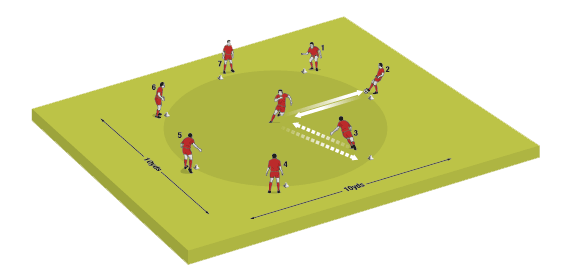
\includegraphics[width=\textwidth]{../img/Trimmed/Clocks1}
        \vspace{12pt}
        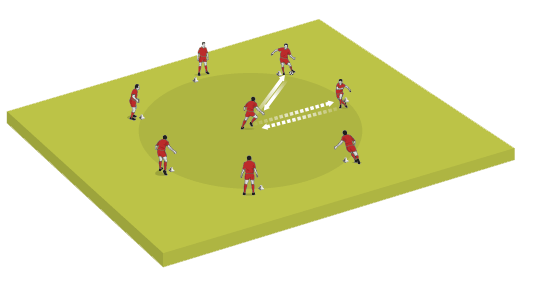
\includegraphics[width=\textwidth]{../img/Trimmed/Clocks2}
    \end{minipage}
    \hspace{0.05\linewidth}
    \begin{minipage}{.6\linewidth} % Left column and width
        \textbf{Drill Description:}
        Create a circle with your players of around 10 yards in diameter. Place cones around the circle where each player should stand, or go inside the centre circle and get the players to take a few steps forwards to get the right size. We’ve used eight players.
        \begin{enumerate}
        \setlength{\itemsep}{0pt}
        \setlength{\parskip}{0pt}
        \setlength{\parsep}{0pt}
        \item Start with the player in the middle who passes to one of the players around the circle
        \item Immediately the pass gets away, the centre player swaps position with the player clockwise from the player he passed to.
        \item The player he swaps with must get quickly into the centre to receive the ball and pass it to the next player anti-clockwise around the circle.
        \item Players continue to pass anti-clockwise and swap position with the player clockwise5. Try and get players to use one touch to get the ball around the clock
        \end{enumerate}
        
        \textbf{Coaching Points:}
        \begin{itemize}
        \setlength{\itemsep}{0pt}
        \setlength{\parskip}{0pt}
        \setlength{\parsep}{0pt}
        \item Focus on who gets your pass and then where you need to move.
        \item Attempt to complete this drill using a single touch.
        \end{itemize}

    \end{minipage}
\end{minipage}

\end{evenBlock}

\begin{evenBlock}{Touchdown Passing}
\begin{minipage}[t]{\linewidth}
    \begin{minipage}{.3\linewidth} % Left column and width
        \centering
        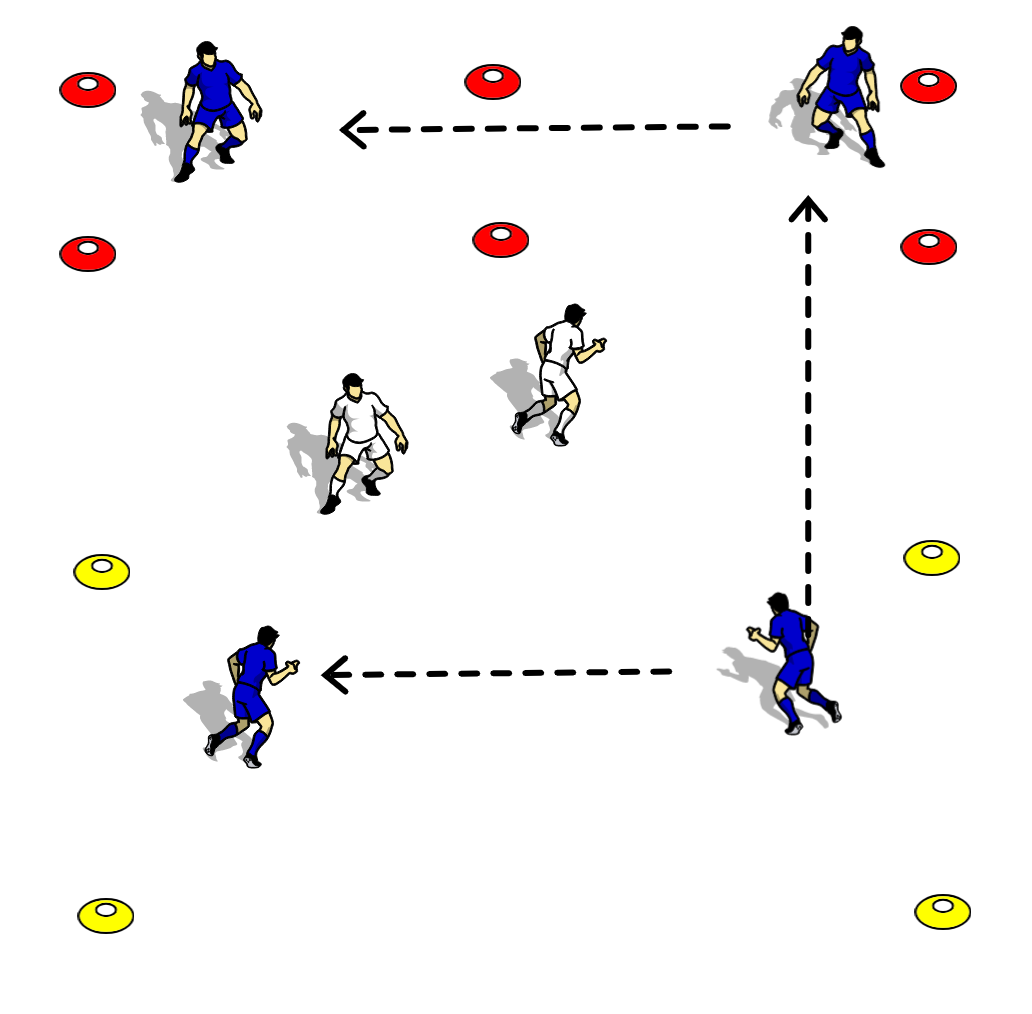
\includegraphics[width=.7\textwidth]{../img/Trimmed/TouchDownPassing}
    \end{minipage}
    \hspace{0.05\linewidth}
    \begin{minipage}{.6\linewidth} % Left column and width
        \textbf{Drill Description:}
        This drill requires 3 pairs of boys.  Pair one are receivers in the end zone.  The second pair are defenders and the last pair are the `quarterbacks' (passers).  The ball starts in the end zone and is passed out to an open passer.  That passer then passes to their partner or back into the touchdown zone. The defenders try and intercept the pass, if they do it successfully, they become the passers and the passers become the defenders.  If the end zone players (receivers pass the ball out of bounds they become the defenders and the defense becomes the receivers.)

        \textbf{NOTE: 2v2 in the box may be hard for new players - try including only 1 defender for a 2v1 passing case as the decision and movement improves add a another defender for a 2v2 situation.}

        %\begin{enumerate}
        %    \setlength{\itemsep}{0pt}
        %    \setlength{\parskip}{0pt}
        %    \setlength{\parsep}{0pt}
        %    \item All players stand `open' so they can see the other two players.
        %    \item The ball should be passed on one direction to start (to the left is more natural for a right footed player).
        %    \item The player receiving the ball should move his body so he receives the ball on his left foot then passes it to the next player using his right.  However the pass should wait until the 3 player is in position.
        %    \item  Player 3 (P3) was at a corner nearest the ball, however once the ball was passed, P3 needs to move to the other corner so they are again at a corner adjacent to the player with the ball.
        %    \item After 5 rounds around the box, switch directions.  Pass to the right using the left foot, trap with the right.
        %    \item After 5 additional rounds allow the player to switch directions at will, but any two adjacent players can't pass the ball back and forth more than 3 times.
        %\end{enumerate}
    \end{minipage}
\end{minipage}
\raggedright
    \textbf{Coaching Points:}
    \begin{itemize}
        \setlength{\itemsep}{0pt}
        \setlength{\parskip}{0pt}
        \setlength{\parsep}{0pt}
        \item Explain the first touch with the correct foot is the most important part.
        \item The touch should place the ball one step away from the player so they can step into and make a strong pass.
        \item The goal is to use two touches, not 1 and not 3.
    \end{itemize}

\end{evenBlock}

\section{Dribbling}
\begin{evenBlock}{Cone Weave Dribbling (10 min)}


\begin{minipage}[t]{\linewidth}
    \centering
    
    \begin{minipage}{.3\linewidth} % Left column and width
        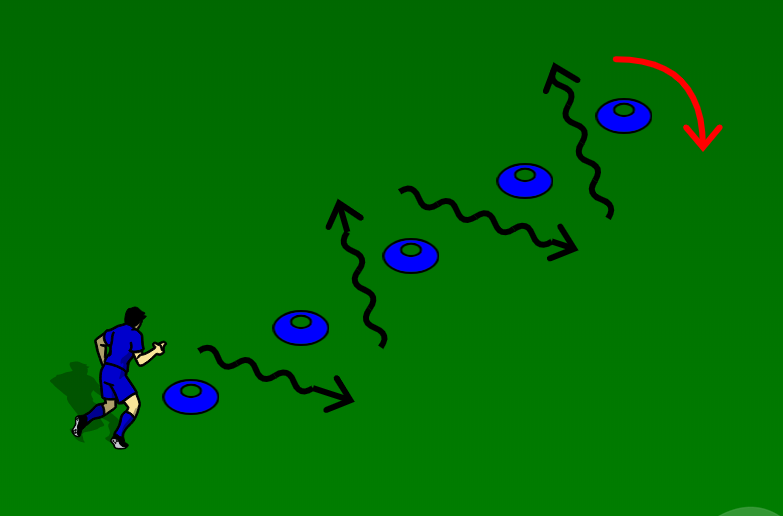
\includegraphics[width=\textwidth]{../img/Trimmed/cone_dribbling}
    \end{minipage}
    \hspace{0.05\linewidth}
    \begin{minipage}{.6\linewidth} % Left column and width
        \textbf{Drill Description:}
        Dribble around 6 cones about 1 yard apart, using only the inside portion of the foot to make cuts.  Ends are different color, orange inside cut, green outside cut.  Players should focus on using 3 touches to make the turn around the end cones.

        \vspace{3pt}
        
        Advanced - use only the outside of the foot or alternate inside foot one direction, outside foot when traveling the other direction.
        %\end{enumerate}

        \vspace{10pt}
        
        \textbf{Coaching Points:}
        \begin{itemize}
        \setlength{\itemsep}{0pt}
        \setlength{\parskip}{0pt}
        \setlength{\parsep}{0pt}
        \item Go slow at first and work up speed as control increases.
        \item Control should be the focus of this drill.  As control increases, increase speed.
        \item Players should always be on their toes, no standing flat footed.
        \item Its better to have 3-5 small controlled touches around the last cone than 3 large out of control touches.
        \end{itemize}

    \end{minipage}
\end{minipage}

\end{evenBlock}

%\begin{evenBlock}{Gate Dribbling (10 min)}
%Set up 3 gates in a zig-zag pattern about 6 to 10 yards apart.  The gates should be about a yard wide or less depending on dribbling skill of the group.  Players start a the end line and dribble through the gates as fast as possible.  Use the same technique as the previous drill.
%\end{evenBlock}

\begin{oddBlock}{Gate Dribbling (10 min)}

\begin{minipage}[t]{\linewidth}
    \centering
    
    \begin{minipage}{.3\linewidth} % Left column and width
        %\begin{figure}
            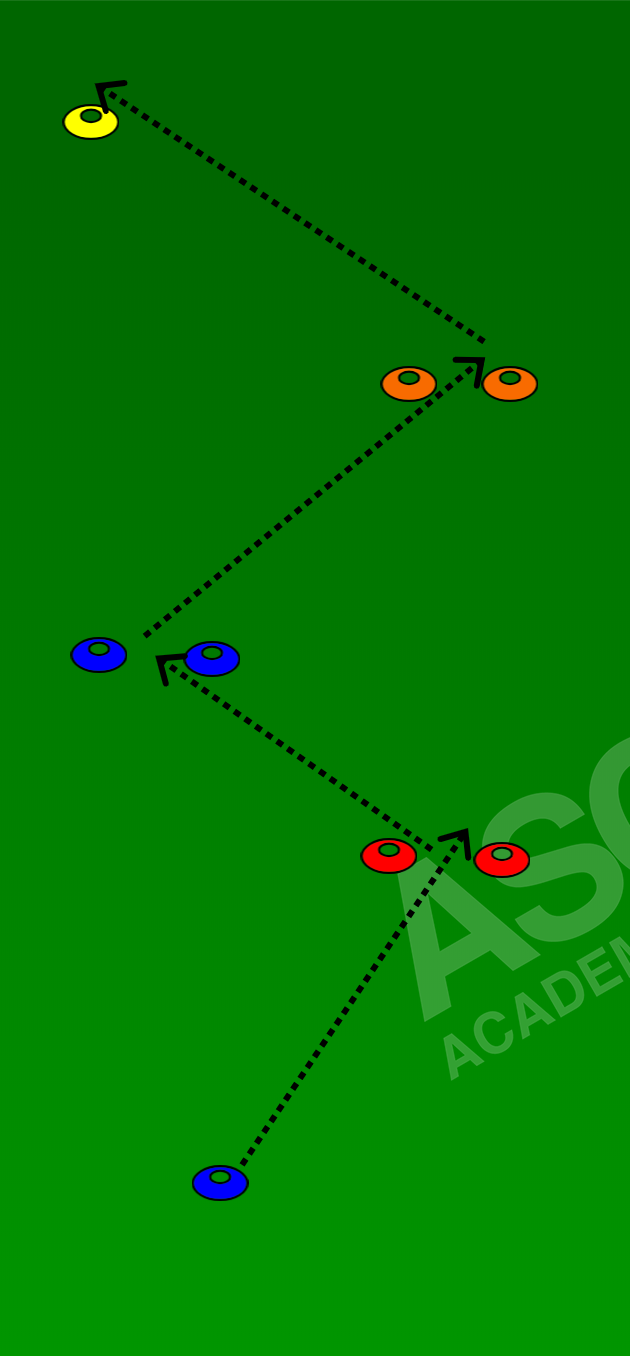
\includegraphics[width=.6\textwidth]{../img/Trimmed/Gate_Dribbling}
        %    \caption{Drill: 4 Person Passing}
        %\end{figure}
    \end{minipage}
    \hspace{0.05\linewidth}
    \begin{minipage}{.6\linewidth} % Left column and width
        \textbf{Drill Description:}
        The object is to dribble at full speed through 3 narrow gates set in a zig-zag pattern about 6 to 10 yards apart.  The gates should be about a yard wide or less depending on dribbling skill of the group.  Once they explode past the yellow cone, they jog back to the end of the line.  Use speed dribbling technique.
        \begin{enumerate}
        \setlength{\itemsep}{0pt}
        \setlength{\parskip}{0pt}
        \setlength{\parsep}{0pt}
        \item Players start at blue gate
        \item Then dribble the ball through the gates.
        \item Once they dribble through the orange gate they explode past the yellow cone.
        \item Then jog back to the end of the line.
        \end{enumerate}

        \textbf{Coaching Points:}
        \begin{itemize}
        \setlength{\itemsep}{0pt}
        \setlength{\parskip}{0pt}
        \setlength{\parsep}{0pt}
        \item When first starting, it will help to focus on proper technique over speed.  Increase the speed as the their technique improves.
        \item Technique uses top outside of the foot, toe down, pushing the ball forward 2 or 3 steps.
        \item Set width of of the gate based on skill.
        \end{itemize}

    \end{minipage}
\end{minipage}

\end{oddBlock}

\section{Defense}
\begin{evenBlock}{Secure the Box}

\begin{minipage}[t]{\linewidth}
    \centering
    
    \begin{minipage}{.3\linewidth} % Left column and width
        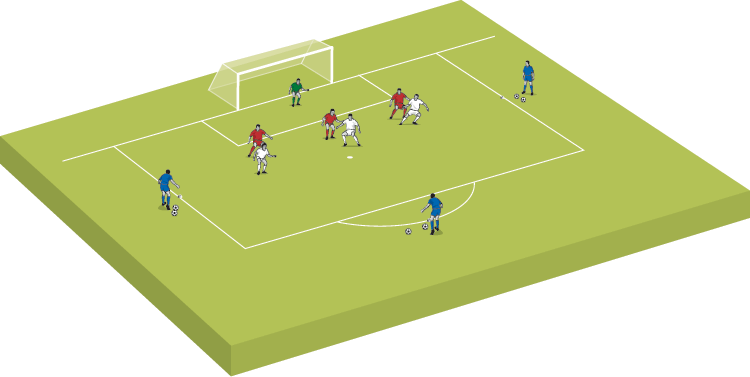
\includegraphics[width=\textwidth]{../img/Trimmed/SecureTheBox1}
    \end{minipage}
    \hspace{0.05\linewidth}
    \begin{minipage}{.6\linewidth} % Left column and width
        \textbf{Drill Description:}
        This drill is ideally played with 9 players, with 3 players per team.  With unbalanced numbers a 4th attacker could be added to create a 4v3 situation to make it harder on the defense (since this is a defensive drill).
        \begin{enumerate}
            \setlength{\itemsep}{0pt}
            \setlength{\parskip}{0pt}
            \setlength{\parsep}{0pt}
            \item The defending team must man mark, with each player picking up an attacker.
            \item The players on the edge of the area have two balls each to pass to the attackers.
            \item The serving players must pass into an attacker who is open (unmarked).
        \end{enumerate}
        
        \textbf{Coaching Points:}
        \begin{itemize}
            \setlength{\itemsep}{0pt}
            \setlength{\parskip}{0pt}
            \setlength{\parsep}{0pt}
            \item Explain marking a player is to remain within 2 or 3 feet of the attackign player.
            \item Explain how to mark a player goal side (defender between the attacker and goal).
            \item Explain how to mark a player ball side (defender between the attacker and the ball).
            \item Explain how to mark a player both goal side and ball side - defender marks the attacker goal side but is a few feet (steps) closer to the ball than the attacker.
            \item Attackers try to lose their marks.  Defenders stay marking the attacker.
            \item Defenders should communicate if they want to defend a zone or a man.  Explain to them how this can work.
            \item If zone defense is too difficult at this stage force them to play man coverage - always marking the same attacker.
        \end{itemize}

    \end{minipage}
\end{minipage}

\end{evenBlock}

\begin{evenBlock}{Foot Soldiers (10 min)}

\begin{minipage}[t]{\linewidth}
    \centering
    
    \begin{minipage}{.4\linewidth} % Left column and width
        \centering
        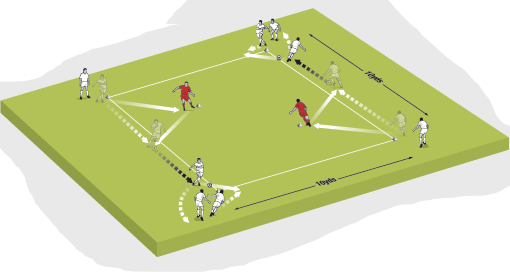
\includegraphics[width=\textwidth]{../img/Trimmed/FootSoldiers1}
        \vspace{6pt}
        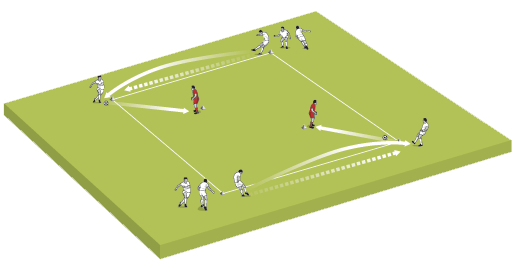
\includegraphics[width=\textwidth]{../img/Trimmed/Footsoldiers2}
    \end{minipage}
    \hspace{0.05\linewidth}
    \begin{minipage}{.5\linewidth} % Left column and width
        \textbf{Drill Description:}
        To use this simple warm-up mark out a 10x10-yard square with cones. Position a cone as shown for the central players. We have used 14 players in this activity, including two servers. You need balls and cones.
        \begin{enumerate}
        \setlength{\itemsep}{0pt}
        \setlength{\parskip}{0pt}
        \setlength{\parsep}{0pt}
        \item Place the two servers inside the square and arrange the remaining players around the four corners of the area use the central players to make one-two wall passes on opposite sides of the square and a first-time pass along the other sides of the square.
        \item Players should sidefoot their passes to the central players, who must make sure that they control the ball and pass it back to the running players so they don’t have to break their stride.
        \item You should swap the players over regularly, changing the two central wall passers. You must have two balls in play at once.
        \end{enumerate}

        \begin{enumerate}
        \setlength{\itemsep}{0pt}
        \setlength{\parskip}{0pt}
        \setlength{\parsep}{0pt}
        \item Play starts on both sides with a pass to the server who plays a one-two with the working player
        \item The player dribbles towards the cone and passes to the player at the cone
        \item The player at the next cone must be on the move to receive the ball and make a one touch pass to the next cone
        \item Players must follow the pass and keep moving around the square
        \item The receiving player for the one-two pass can take two touches because this needs to be an accurate move with a good weight on the pass
        \end{enumerate}

    \end{minipage}
\end{minipage}

\end{evenBlock}

\begin{evenBlock}{Block Passing}

\begin{minipage}[t]{\linewidth}
    \centering
    
    \begin{minipage}{.4\linewidth} % Left column and width
        \centering
        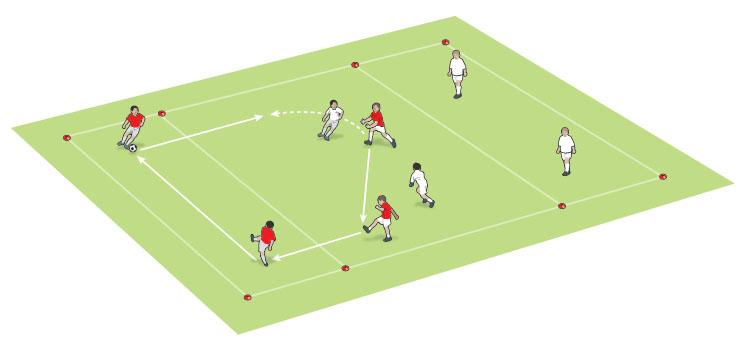
\includegraphics[width=\textwidth]{../img/Trimmed/Block_Passing_1}
        \vspace{6pt}
        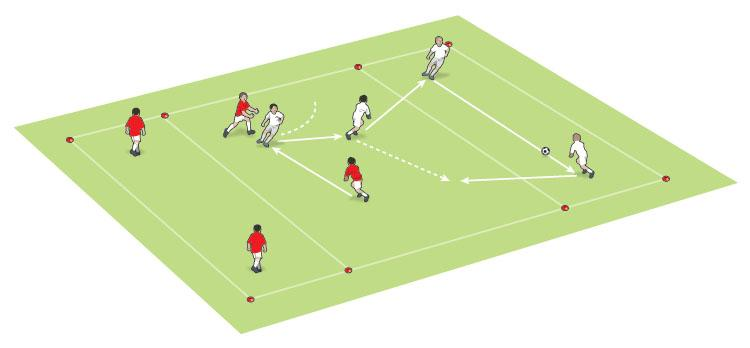
\includegraphics[width=\textwidth]{../img/Trimmed/Block_Passing_2}
    \end{minipage}
    \hspace{0.05\linewidth}
    \begin{minipage}{.5\linewidth} % Left column and width
        \textbf{Drill Description:}
        A drill that focuses on pressing and avoiding the press.  The goal is to keep the ball as long as possible.
        
        \begin{enumerate}
        \setlength{\itemsep}{0pt}
        \setlength{\parskip}{0pt}
        \setlength{\parsep}{0pt}
        \item This is a 4v4 game.
        \item 20x15 yard area with two 5 yard end zones.
        \item The end zones are safe zones and are occupied with 2 teammates.
        \item The other 2 teammates from each team are in the central zone playing 2v2 keep away.
        \item The center players can pass to the end zone players who are safe from attack, but only after they successully passed it within the central zone.
        \end{enumerate}

        \textbf{Coaching Points:}
        \begin{enumerate}
        \setlength{\itemsep}{0pt}
        \setlength{\parskip}{0pt}
        \setlength{\parsep}{0pt}
        \item Where are you passing options?
        \item Support your teammate.
        \item Know where the ball is!
        \item Block the ball or the pass.  Know where your team is.
        \item Without the ball move and talk so your partner knows where you are without seeing you.
        \end{enumerate}
    \end{minipage}
\end{minipage}

\end{evenBlock}

\begin{evenBlock}{Press \& Protect}

\begin{minipage}[t]{\linewidth}
    \centering
    
    \begin{minipage}{.4\linewidth} % Left column and width
        \centering
        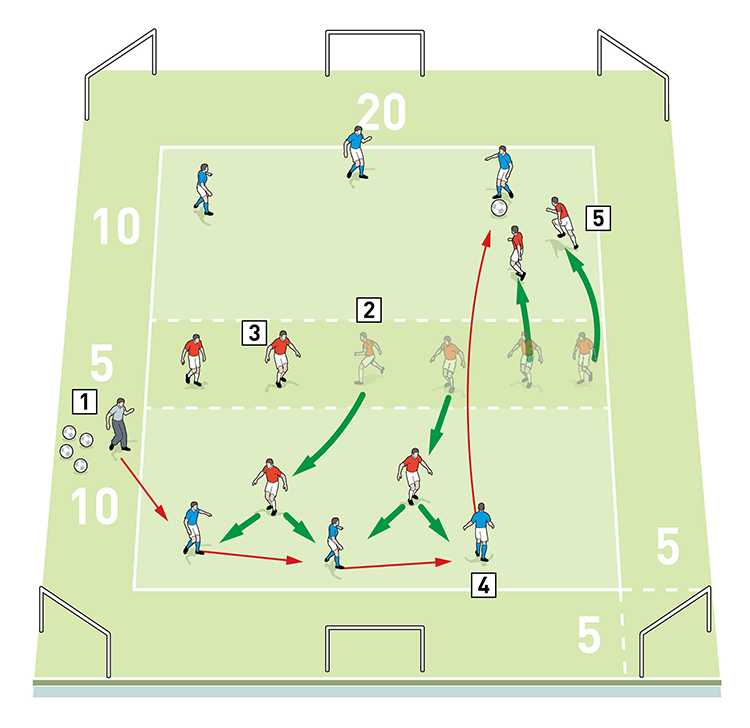
\includegraphics[width=\textwidth]{../img/Trimmed/Press_Protect}

        \vspace{6pt}
        
        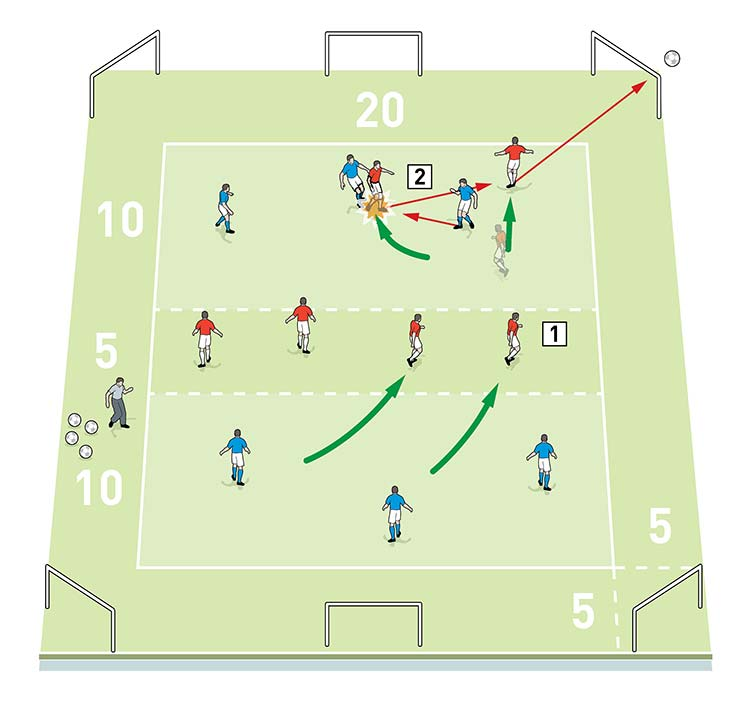
\includegraphics[width=\textwidth]{../img/Trimmed/Press_Protect_2}
    \end{minipage}
    \hspace{0.05\linewidth}
    \begin{minipage}{.5\linewidth} % Left column and width
        \textbf{Drill Description:}
        A drill that focuses on pressing and quick decision making for the passing team.  It also works on showing the importance of the center field player in their role of blocking through balls.
        
        \begin{enumerate}
        \setlength{\itemsep}{0pt}
        \setlength{\parskip}{0pt}
        \setlength{\parsep}{0pt}
        \item 20x25 yard area with a 5 yard middle zone.
        \item The pressing team of 6 stage in the middle, the other team (defending team) splits into 2 groups of 3 in on 10x20 side areas.
        \item 6 goals are positioned around 5 yard outside the area - the pressing team can score by passing the ball through any of these 6 goals.
        \item Coach is on the side line passing balls in.
        \item The pressing team is trying to score goals.
        \item The defending team is playing keep away and can pass to the other side.  At which point the press has to return to the center box 2 other players from the center box come out to press the other side.
        \item Switch roles every 5 minutes or 1/4 of the allocated time.
        \end{enumerate}

        \textbf{Coaching Points:}
        \begin{enumerate}
        \setlength{\itemsep}{0pt}
        \setlength{\parskip}{0pt}
        \setlength{\parsep}{0pt}
        \item Make quick passes.
        \item Think where should I pass the ball all the time (especially when the ball is not at your feet).
        \end{enumerate}
    \end{minipage}
\end{minipage}

\end{evenBlock}

\section{Game Situational}
\begin{evenBlock}{Outside Forward Drive to Endline and Cross (10 min)}

\begin{minipage}[t]{\linewidth}
    \centering
    
    \begin{minipage}{.3\linewidth} % Left column and width
        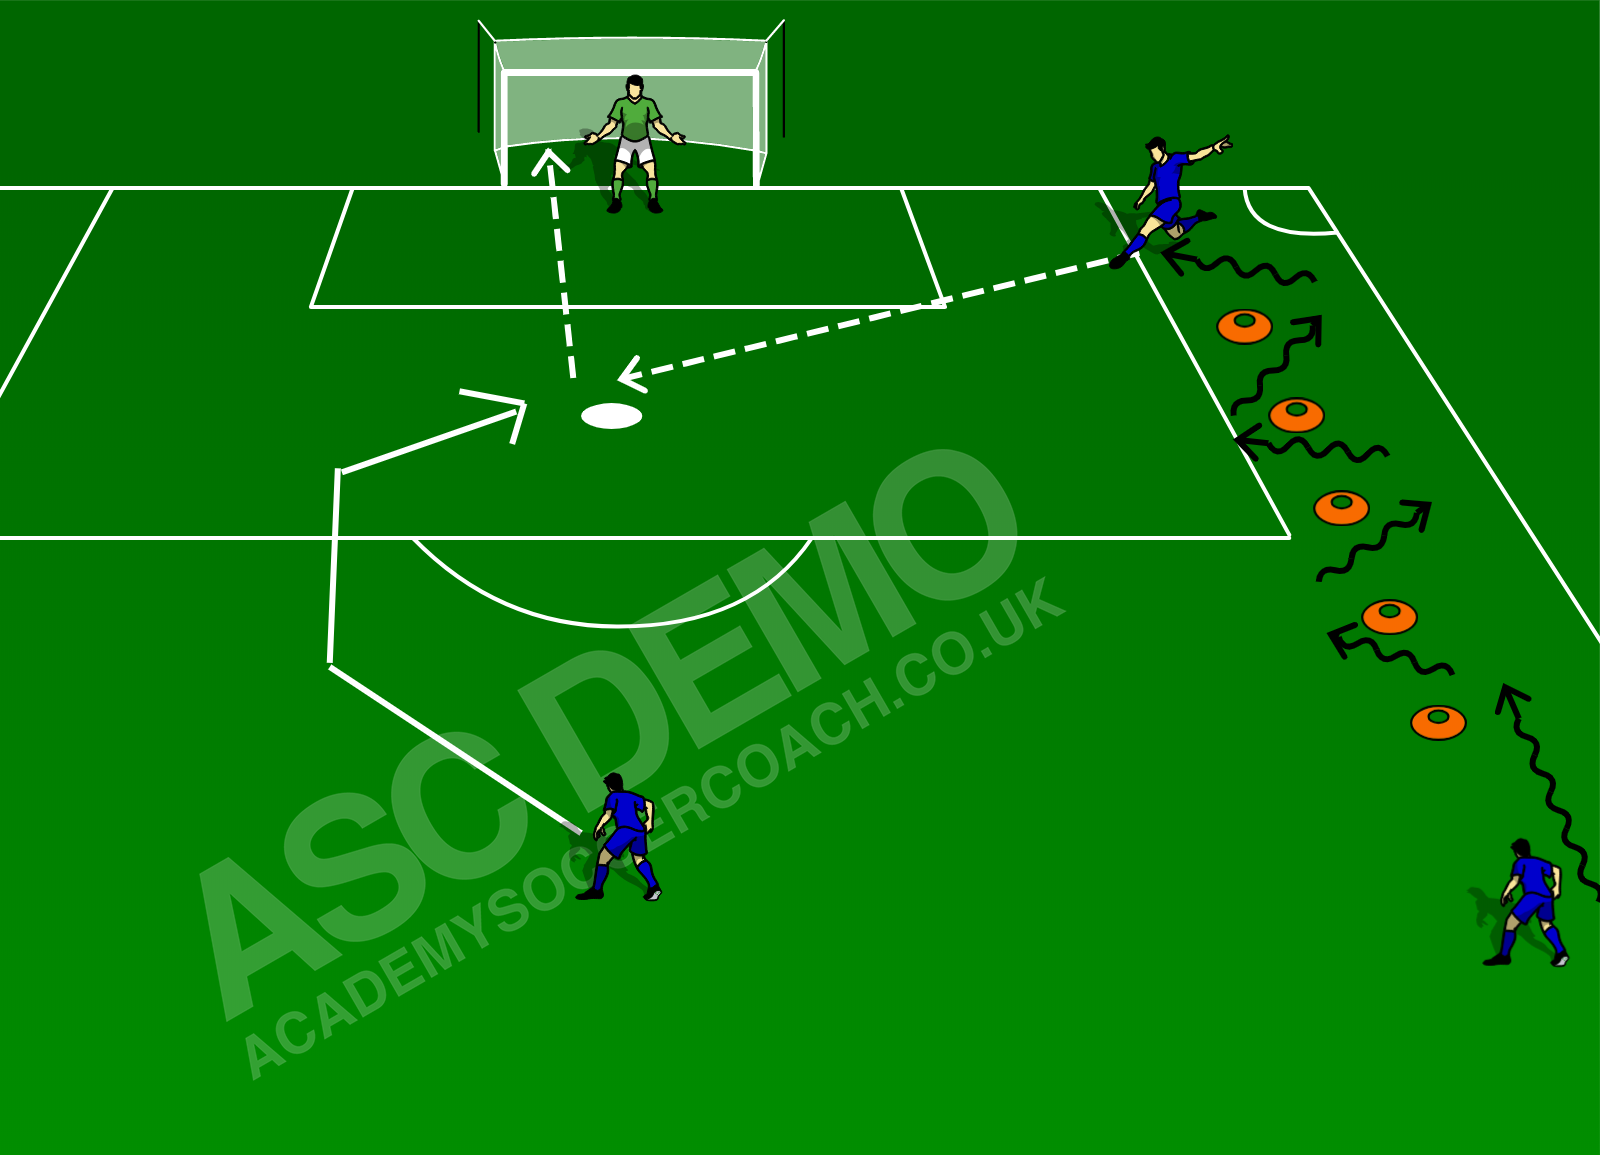
\includegraphics[width=\textwidth]{../img/Trimmed/Dribble-Cross-Shoot}
    \end{minipage}
    \hspace{0.05\linewidth}
    \begin{minipage}{.6\linewidth} % Left column and width
        \textbf{Drill Description:}
        \begin{enumerate}
        \setlength{\itemsep}{0pt}
        \setlength{\parskip}{0pt}
        \setlength{\parsep}{0pt}
        \item A line forms at half field, with a set of balls.
        \item Player 1 dribbles through cones, turning around the last cone toward goal,
        \item P1 then crosses the ball to the PK spot where the Striker takes his one touch shot.
        \item Striker retrieves the ball and goes to the end of the line.
        \item Wing then shifts to the striker role.
        \end{enumerate}

        \vspace{6pt}
        
        Once everyone goes once or twice switch side of the field and uses left feet for crossing and shooting.

        \vspace{6pt}
        
        Playing a Keeper is optional.

        \vspace{10pt}
        
        \textbf{Coaching Points:}
        \begin{itemize}
        \setlength{\itemsep}{0pt}
        \setlength{\parskip}{0pt}
        \setlength{\parsep}{0pt}
        \item The touch around that last cone is the most important. 
        \item Body position around that last cone is critical as well.  The players hips need to be tuned toward the PK spot otherwise the player gives up both power and control over the pass.
        \item The striker must be patient and not over run the spot.  Move in an arc away from center, then back toward the ball.  Accelerate once the ball is passed and kick it into goal.
        \end{itemize}

    \end{minipage}
\end{minipage}

\end{evenBlock}

\begin{evenBlock}{2 vs. 1 Offense (10 min)}


\begin{minipage}[t]{\linewidth}
    \centering
    
    \begin{minipage}{.3\linewidth} % Left column and width
        %\begin{figure}
            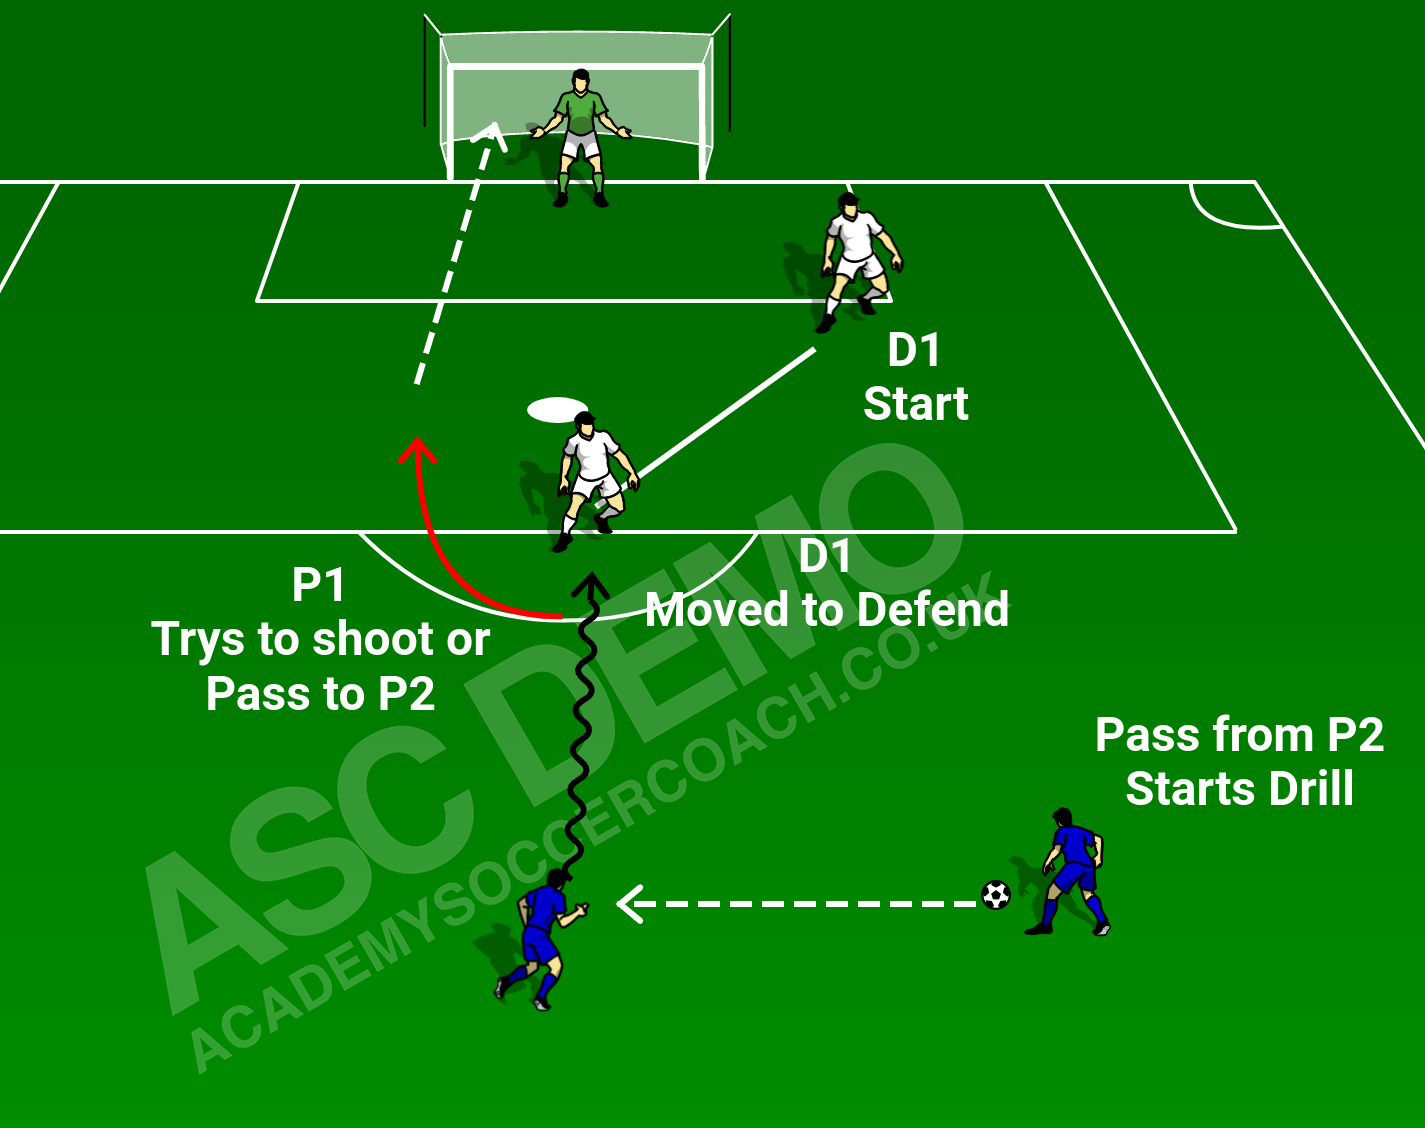
\includegraphics[width=\textwidth]{../img/Trimmed/2v1_Option}

            \vspace{3pt}
            
            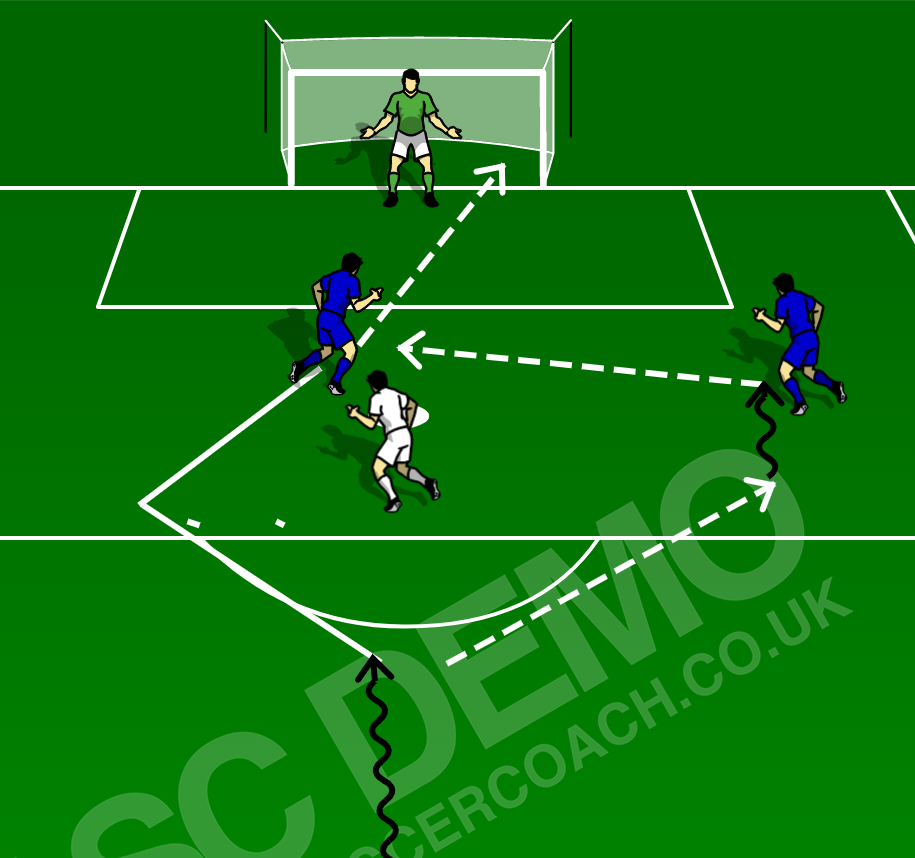
\includegraphics[width=\textwidth]{../img/Trimmed/2v1_Option_Pass}
        %    \caption{Drill: 4 Person Passing}
        %\end{figure}
    \end{minipage}
    \hspace{0.05\linewidth}
    \begin{minipage}{.6\linewidth} % Left column and width
        \textbf{Drill Description:}
        This drill is designed train the forward to make a quick decision on how to beat a defender.  He has two options, dribble around the defender or pass to his wing and make a move around the defender. 
        \begin{enumerate}
        \setlength{\itemsep}{0pt}
        \setlength{\parskip}{0pt}
        \setlength{\parsep}{0pt}
        \item The wing (P2) starts the play by passing to the forward.  The defender (D1) starts at the corner of the 6 yard box.
        \item The forward drives to goal as a defender come charging to defend.
        \item The forward has two choices, pass or make a move/touch around the defender.
        \item The goal is to get a shot on goal.
        \item If he passes the ball, the wing should cross the ball quickly as the striker is passing the defender.
        \end{enumerate}

        \vspace{3pt}
        
        Rotate rolls each shot: P2 to P1, P1 to D1, D1 to P2.

        \vspace{10pt}
        
        \textbf{Coaching Points:}
        \begin{itemize}
        \setlength{\itemsep}{0pt}
        \setlength{\parskip}{0pt}
        \setlength{\parsep}{0pt}
        \item The forward needs to decide quickly which option he plans to take.
        \item The wing needs to be ready at all times and should stay `on-side'.
        \item The forward should try and take advantage of any weakness of the defense, or try and create weakness by using a scissor move or a fake.
        \item Explain on-sides and off-sides.
        \end{itemize}

    \end{minipage}
\end{minipage}

\end{evenBlock}

\begin{evenBlock}{3+Help vs. 4}

\begin{minipage}[t]{\linewidth}
    \centering
    
    \begin{minipage}{.3\linewidth} % Left column and width
        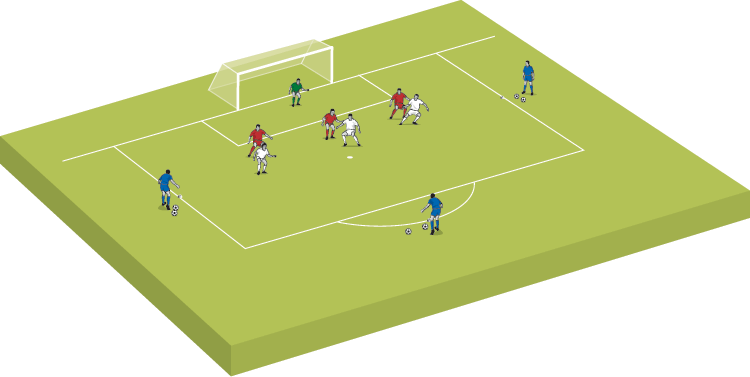
\includegraphics[width=\textwidth]{../img/Trimmed/SecureTheBox1}
    \end{minipage}
    \hspace{0.05\linewidth}
    \begin{minipage}{.6\linewidth} % Left column and width
        \textbf{Drill Description:}
        This drill is ideally played with 10 players, 4 defensive players + 1 keeper and 5 attacking players.  Thsi uses one half the field, the 3 Attacking players start that the mid field line.  Two mid fielders are on the defensive side of the midfield line.  The mid fielders can't cross the line, they can be passed to and then pass back to one of the three forwards or the other mid fielder.  The striker starts the drill by passing to one of his wings.  The 4 defensive backs guard the box and once the ball is passed can move to defend.  Defense wins if the ball is cleared.  Offense wins if they score or win a corner kick.
        
        \textbf{Coaching Points:}
        \begin{itemize}
            \setlength{\itemsep}{0pt}
            \setlength{\parskip}{0pt}
            \setlength{\parsep}{0pt}
            \item Remind the defense about the funnel positioning.
            \item Explain how to mark a player goal side (defender between the attacker and goal).
            \item Explain how to mark a player ball side (defender between the attacker and the ball).
            \item Explain how to mark a player both goal side and ball side - defender marks the attacker goal side but is a few feet (steps) closer to the ball than the attacker.
            \item Defenders should communicate if they want to defend a zone or a man.  Explain to them how this can work.
            \item Attackers look for open space.
            \item Mid fielders look for open space on the opposite side of the field.
        \end{itemize}

    \end{minipage}
\end{minipage}

\end{evenBlock}

\section{Other}
Double attacker
by Dave Clarke in Attacking, Crossing
PRINT 
In this session the wide player must complete a one-two and overlap to give attackers two ways to score. This is a great for wingers to be coached in different ways to attack from the wings

Set up
Use half your normal pitch. We’ve used 11 players in the session plus a coach to serve. You need balls, bibs, cones and a goal.

How to play
The session starts with the winger A playing a one-two with his team mate and crossing for the attackers. Winger B then receives a ball from the server, passes to winger A and makes an overlapping run to receive a pass and crosses into the box for a new set of attackers. Attackers go to the back of the queue each time. The next double attack comes from the opposite wing. Play for three sets of crosses from both wings then switch players around.

Technique
This is a great session for practising wing play and working combinations that can create goals from fast wingers. It’s also good practice for technique.

Wingers pass to striker

1. Play starts with a one-two between winger A and winger B2. Winger A gets the ball back then plays a cross into the path of the oncoming attackers
score from crosses

3. The server then plays a second ball to B who sends A down the line with a pass4. B waits for the run of A and times a good pass down the wing to take the ball in his stride


5. The overlapping B runs around A and receives the ball to pass into the feet of the advancing attackers

%\begin{evenBlock}{Gate Dribbling (10 min)}
%Set up 3 gates in a zig-zag pattern about 6 to 10 yards apart.  The gates should be about a yard wide or less depending on dribbling skill of the group.  Players start a the end line and dribble through the gates as fast as possible.  Use the same technique as the previous drill.
%\end{evenBlock}

\begin{oddBlock}{De-Acceleration Shuddle}

\begin{minipage}[t]{\linewidth}
    \centering
    
    \begin{minipage}{.3\linewidth} % Left column and width
        %\begin{figure}
            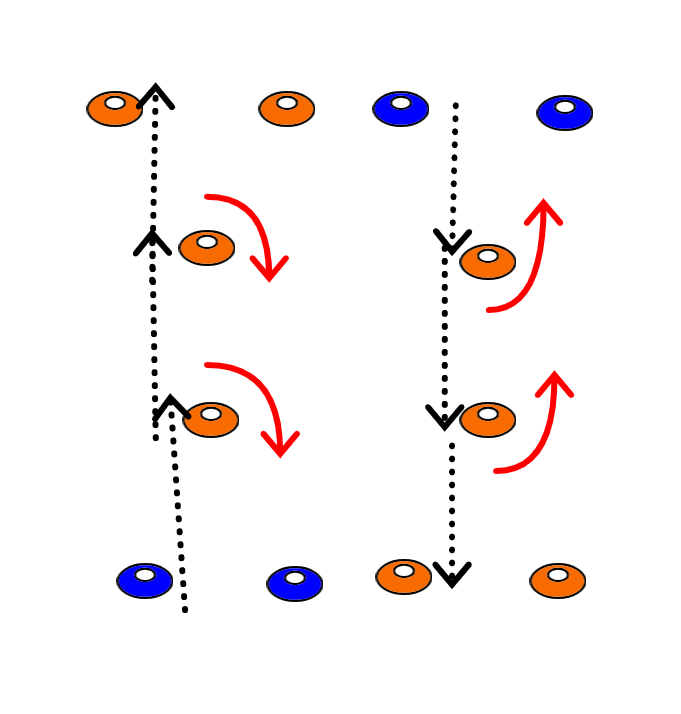
\includegraphics[width=\textwidth]{../img/Trimmed/deaccel_shuddle}
        %    \caption{Drill: 4 Person Passing}
        %\end{figure}
    \end{minipage}
    \hspace{0.05\linewidth}
    \begin{minipage}{.6\linewidth} % Left column and width
        \textbf{Drill Description:}
        This is an agility drill to practice both acceleration and de-acceleration.
        \begin{enumerate}
        \setlength{\itemsep}{0pt}
        \setlength{\parskip}{0pt}
        \setlength{\parsep}{0pt}
        \item Players start at blue gate
        \item Then run to the left hand side of the first orange cone and while facing forward shuddle around the cone using at least 6 quick toe taps.
        \item Then accelerate to the left of the next orange cone and shuddle around the cone then finish with a full acceleration through the orange gate.
        \item A second line forms behind the other blue cone and the drill repeats but this time one races to the right hand side of the cones and shuddle around to the left.
        \item Repeat each set 4 times.
        \end{enumerate}
    \end{minipage}
\end{minipage}
    \vspace{12pt}
    
    \textbf{Coaching Points:}
    \begin{itemize}
        \setlength{\itemsep}{0pt}
        \setlength{\parskip}{0pt}
        \setlength{\parsep}{0pt}
        \item Focus on quickly getting to speed then slowing down.
        \item Focus on using small quicks touches around the cone, keeping it tight.
        \item Stay low and use your bend legs to explode away,
        \item Then compress them to slow down.
        \item Finish strong by sprinting right through the last gate, jogging back to the next blue gate.
    \end{itemize}
\end{oddBlock}

%\begin{evenBlock}{Gate Dribbling (10 min)}
%Set up 3 gates in a zig-zag pattern about 6 to 10 yards apart.  The gates should be about a yard wide or less depending on dribbling skill of the group.  Players start a the end line and dribble through the gates as fast as possible.  Use the same technique as the previous drill.
%\end{evenBlock}

\begin{oddBlock}{Lateral Shuttle}

\begin{minipage}[t]{\linewidth}
    
    \begin{minipage}{.2\linewidth} % Left column and width
        \centering
        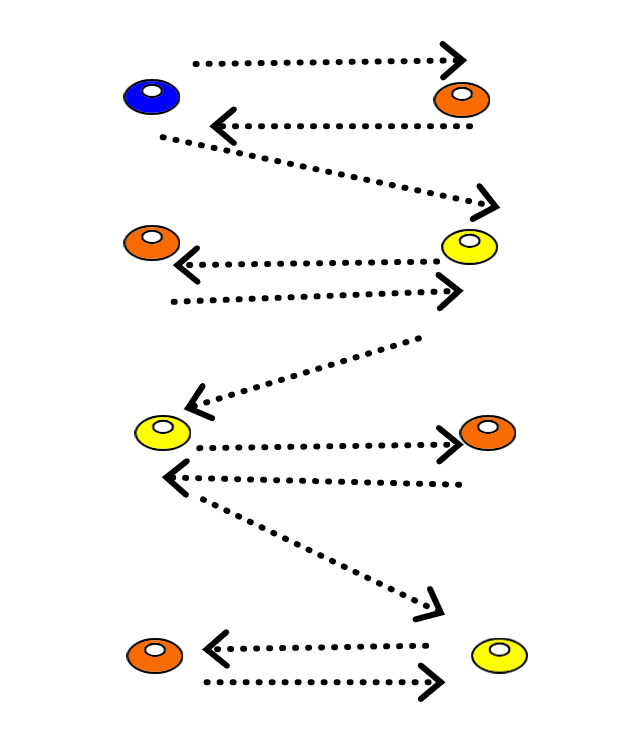
\includegraphics[width=\textwidth]{../img/Trimmed/lateral_shuddle}
    \end{minipage}
    \hspace{0.05\linewidth}
    \begin{minipage}{.7\linewidth} % Left column and width
        \textbf{Drill Description:}
        This agility drill works on lateral shuffling a critical skill for defenders. 
        \begin{enumerate}
            \setlength{\itemsep}{0pt}
            \setlength{\parskip}{0pt}
            \setlength{\parsep}{0pt}
            \item Players start at blue gate facing the line of 3 cones ahead of him,
            \item They shuttle side-ways to the orange cone, touch it with a finger then shuttle back to the blue cone touching it.
            \item Shuttle to diagonally to the yellow cone then to the orange cone, touching it, and back then to the yellow cone touching it, then shuttle diagonally to the next yellow cone.
            \item Keep repeating until the end.
        \end{enumerate}
    \end{minipage}
\end{minipage}
    %\vspace{12pt}
    %
    %\textbf{Coaching Points:}
    %\begin{itemize}
    %    \setlength{\itemsep}{0pt}
    %    \setlength{\parskip}{0pt}
    %    \setlength{\parsep}{0pt}
    %    \item TBD
    %\end{itemize}
\end{oddBlock}

%\begin{evenBlock}{Gate Dribbling (10 min)}
%Set up 3 gates in a zig-zag pattern about 6 to 10 yards apart.  The gates should be about a yard wide or less depending on dribbling skill of the group.  Players start a the end line and dribble through the gates as fast as possible.  Use the same technique as the previous drill.
%\end{evenBlock}

\begin{oddBlock}{Cross-Hairs}

\begin{minipage}[t]{\linewidth}
    \centering
    
    \begin{minipage}{.2\linewidth} % Left column and width
        
        \centering
        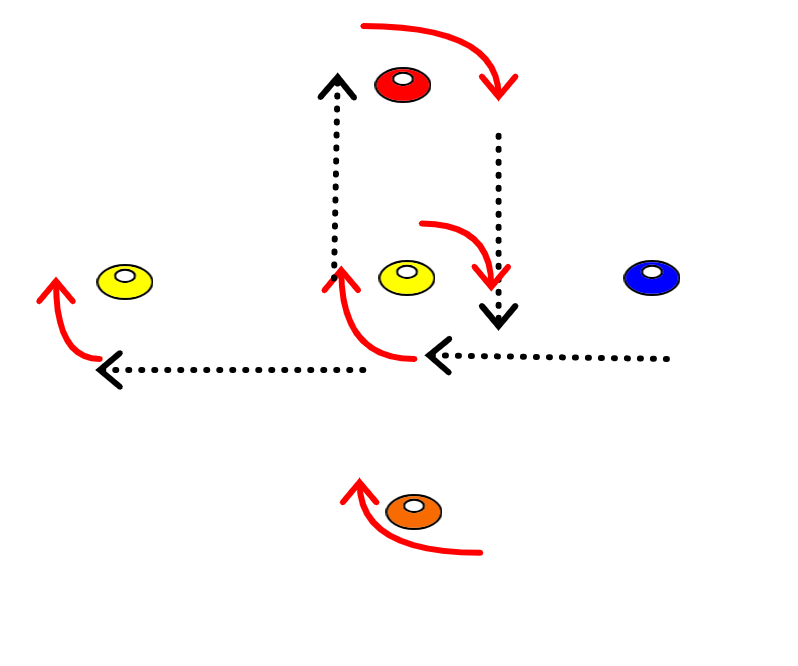
\includegraphics[width=\textwidth]{../img/Trimmed/cross_hairs}

    \end{minipage}
    \hspace{0.05\linewidth}
    \begin{minipage}{.7\linewidth} % Left column and width
        \textbf{Drill Description:}
        
        \begin{enumerate}
        \setlength{\itemsep}{0pt}
        \setlength{\parskip}{0pt}
        \setlength{\parsep}{0pt}
        \item Players start at blue cone and race to the center cone turn right and race around the outer cones and always returning to the center cone.
        \item Finish by accelerating past the blue cone.
        \end{enumerate}
    \end{minipage}
\end{minipage}
%\vspace{12pt}
%
%    \textbf{Coaching Points:}
%    \begin{itemize}
%        \setlength{\itemsep}{0pt}
%        \setlength{\parskip}{0pt}
%        \setlength{\parsep}{0pt}
%        \item
%    \end{itemize}

\end{oddBlock}

\begin{evenBlock}{3v2+Keeper}

\begin{minipage}[t]{\linewidth}
    \centering
    
    \begin{minipage}{.5\linewidth} % Left column and width
        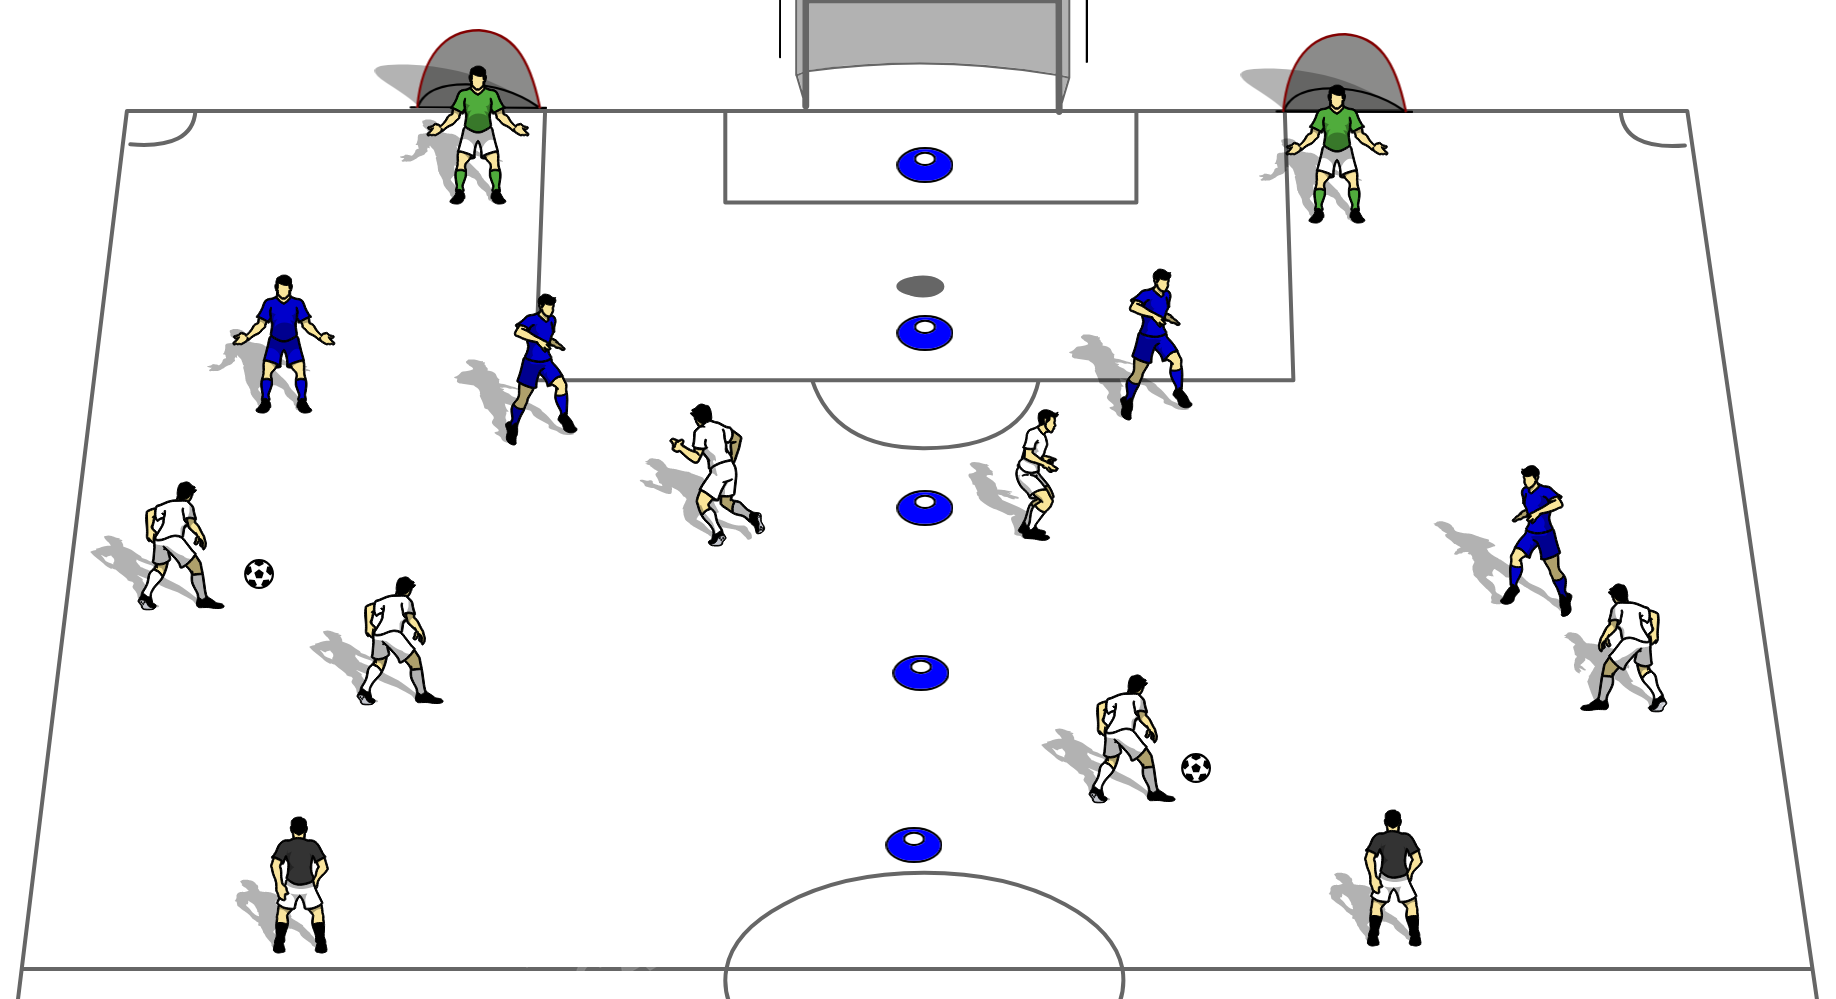
\includegraphics[width=\textwidth]{../img/Trimmed/3v2+Keeper}
    \end{minipage}
    \hspace{0.05\linewidth}
    \begin{minipage}{.4\linewidth} % Left column and width
        \textbf{Drill Description:}
        This drill requires 6 players + 1 coach or 12 players and 2 coaches.
        \begin{enumerate}
            \setlength{\itemsep}{0pt}
            \setlength{\parskip}{0pt}
            \setlength{\parsep}{0pt}
            \item The defending team uses 2 defenders and 1 keeper.
            \item Attacking team has 3 and tries to score on the small defended goal.
            \item The defending team scores by completing a pass to the coach on the center line.
        \end{enumerate}
    \end{minipage}
\end{minipage}
\vspace{12pt}

\textbf{Coaching Points:}
\begin{itemize}
    \setlength{\itemsep}{0pt}
    \setlength{\parskip}{0pt}
    \setlength{\parsep}{0pt}
    \item Explain marking a player is to remain within 2 or 3 feet of the attacking player.
    \item Explain how to mark a player goal side (defender between the attacker and goal).
    \item Attackers try to lose their marks by passing.
\end{itemize}
\end{evenBlock}

\begin{evenBlock}{Get the Snitch}

\begin{minipage}[t]{\linewidth}
    \centering
    
    \begin{minipage}{.5\linewidth} % Left column and width
        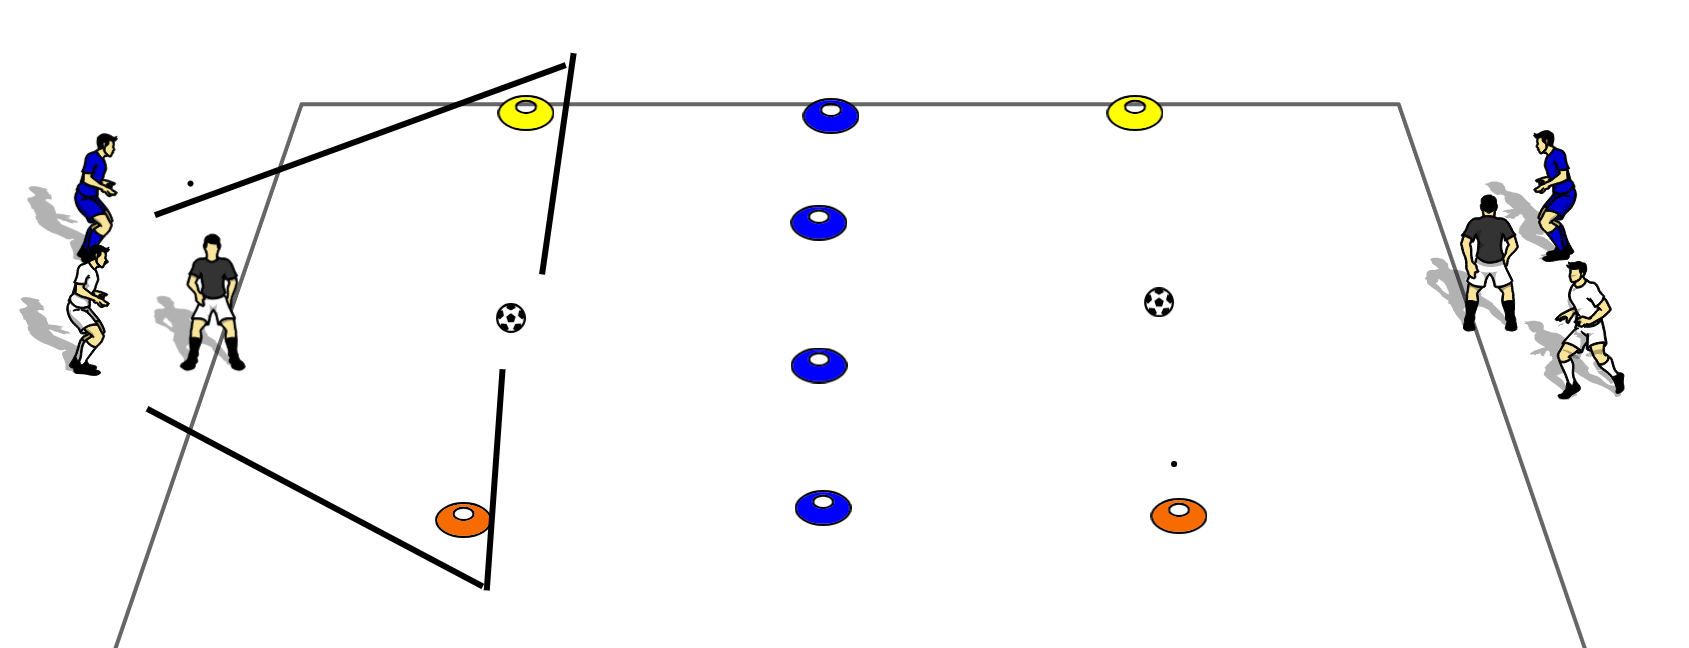
\includegraphics[width=\textwidth]{../img/Trimmed/Get_the_Snitch}
    \end{minipage}
    \hspace{0.05\linewidth}
    \begin{minipage}{.4\linewidth} % Left column and width
        \textbf{Drill Description:}
        The object is to get the ball (the snitch) and take it across the opposite end line.
        \begin{enumerate}
            \setlength{\itemsep}{0pt}
            \setlength{\parskip}{0pt}
            \setlength{\parsep}{0pt}
            \item Coach calls go and kicks a ball into the field, both players race around their cone to get to the ball.
            \item First player to get the ball tries to drive across the fair end line while the other player defends that line.
        \end{enumerate}
    \end{minipage}
\end{minipage}
\vspace{12pt}

%\textbf{Coaching Points:}
%\begin{itemize}
%    \setlength{\itemsep}{0pt}
%    \setlength{\parskip}{0pt}
%    \setlength{\parsep}{0pt}
%    \item Explain marking a player is to remain within 2 or 3 feet of the attacking player.
%    \item Explain how to mark a player goal side (defender between the attacker and goal).
%    \item Attackers try to lose their marks by passing.
%\end{itemize}
\end{evenBlock}

\begin{evenBlock}{1v1 Evade with Help}

\begin{minipage}[t]{\linewidth}
    \centering
    
    \begin{minipage}{.5\linewidth} % Left column and width
        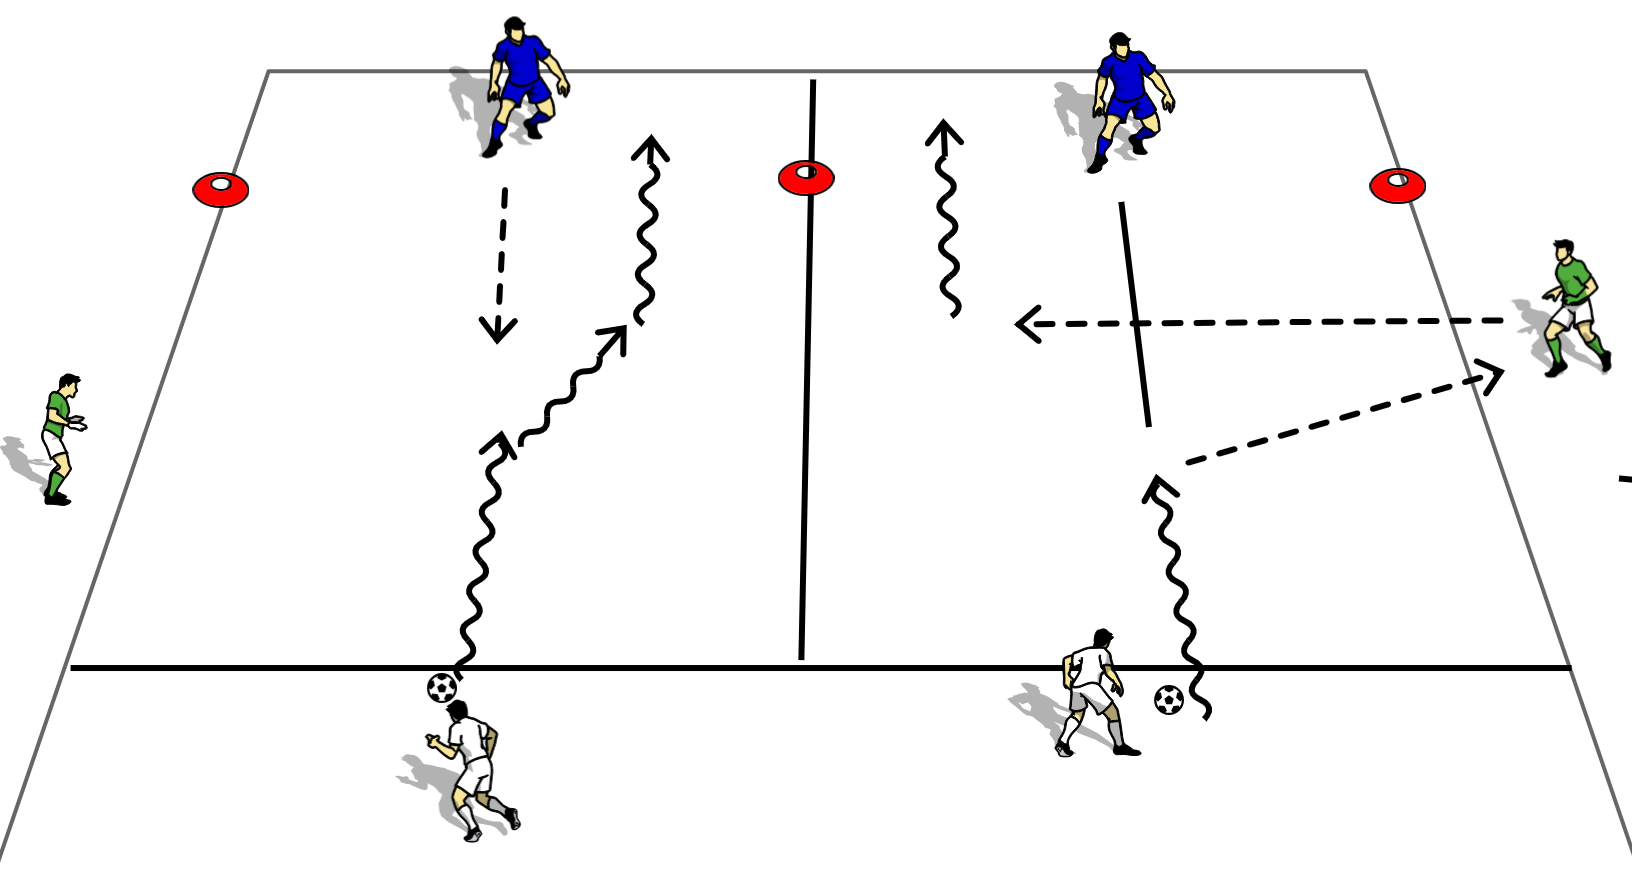
\includegraphics[width=\textwidth]{../img/Trimmed/Evade_1V1+Help}
    \end{minipage}
    \hspace{0.05\linewidth}
    \begin{minipage}{.4\linewidth} % Left column and width
        \textbf{Drill Description:}
        The object is to get the ball (the snitch) and take it across the opposite end line.
        \begin{enumerate}
            \setlength{\itemsep}{0pt}
            \setlength{\parskip}{0pt}
            \setlength{\parsep}{0pt}
            \item Player with the ball crosses the far end line and ties to dribble across the opposite endline.
            \item A defender starts behind the red cones and can cross them as soon as the attacker enters the box.
            \item The attacker needs to evade the defender or pass to his helper (coach) on the side line, who one touches the ball back into play.
        \end{enumerate}
    \end{minipage}
\end{minipage}
\vspace{12pt}

\textbf{Coaching Points:}
\begin{itemize}
    \setlength{\itemsep}{0pt}
    \setlength{\parskip}{0pt}
    \setlength{\parsep}{0pt}
    \item The timing of the attacking move is critical, it needs to be early enough to insure the defender can't block it, but not so early the defender can react to counter it.
    \item Use the pass as a great opportunity to evade the defender.
\end{itemize}
\end{evenBlock}

\end{document}